\documentclass[convert={svg,command=\unexpanded{{inkscape\space --pdf-poppler\space --export-type="svg"\space --pages=1\space -o\space \outfile\space \infile}}}]{standalone}% 'crop' is the default for v1.0, before it was 'preview'

\usepackage{tikz}
\usepackage{pgfplots}
\usepgfplotslibrary{fillbetween}
\usetikzlibrary{patterns, patterns.meta, positioning, math}

\pgfplotsset{compat=1.18}

\usepackage{tikz-3dplot}
\usetikzlibrary{3d,calc}

\pgfplotsset{
	twoDaxis/.style = {
			no marks,
			samples = 100,
			axis lines = center,
			xlabel = {$x$},
			ylabel = {$y$},
			every axis x label/.style={
					at={(ticklabel* cs:1.05)},
					anchor=west,
				},
			every axis y label/.style={
					at={(ticklabel* cs:1.05)},
					anchor=south,
				},
		},
	threeDaxis/.style = {
			axis z line = none,
			axis lines=center, % remove this and you get weird box behavior, not good for calc 2 students
			xlabel=$x$, % you know this one
			every axis x label/.style={
					at={(ticklabel* cs:1.05)},
					anchor=west,
				}, % place the xlabel in a better spot
			ylabel=$y$, % you know this one
			every axis y label/.style={
					at={(ticklabel* cs:1.05)},
					anchor=north,
				}, % places y label in a better spot
		},
	threeDaxiswithyzswap/.style = {
			axis y line = none,
			axis lines=center, % remove this and you get weird box behavior, not good for calc 2 students
			xlabel=$x$, % you know this one
			every axis x label/.style={
					at={(ticklabel* cs:1.05)},
					anchor=west,
				}, % place the xlabel in a better spot
			zlabel=$y$, % you know this one
			every axis z label/.style={
					at={(ticklabel* cs:1.05)},
					anchor=south, % which side of the label gets pinned to the point 5% past the axis end point?
				}, % places y label in a better spot
			xticklabel style = {font=\tiny, yshift=1ex},
			zticklabel style = {font=\tiny, xshift=1ex},
		}
}

\def\centerarc[#1](#2)(#3:#4:#5)% Syntax: [draw options] (center) (initial angle:final angle:radius)
{ \draw[#1] ($(#2)+(axis direction cs:{#5*cos(#3)},{#5*sin(#3)})$) arc (#3:#4:#5); }

\def\centerarc[#1](#2)(#3:#4:#5:#6)% Syntax: [draw options] (center) (initial angle:final angle:xradius:yradius)
{ \draw[#1] ($(#2)+(axis direction cs:{#5*cos(#3)},{#6*sin(#3)})$) arc  [start angle = #3, end angle = #4, x radius = #5, y radius = #6]; }

\def\diskslicevert[#1](#2)(#3:#4)% Syntax: [draw options] (center) (xradius:yradius) use {} if functions on things!!!!!!
{ 		\draw [<->, #1] (#2) -- ($(#2)+(axis direction cs:{0},{#4})$) node [midway, right] {$R$};
	\centerarc[#1](#2)(20:340:{#3}:{#4});
	\centerarc[dotted, #1](#2)(340:380:{#3}:{#4});
}
\def\diskslicevert[#1,r=#2](#3)(#4:#5)% Syntax: [draw options] (center) (xradius:yradius)
{ 		\draw [<->, #1] (#3) -- ($(#3)+(axis direction cs:{0},{#5})$) node [midway, right] {#2};
	\centerarc[#1](#3)(20:340:{#4}:{#5});
	\centerarc[dotted, #1](#3)(340:380:{#4}:{#5});
}
\def\diskslicevertflip[#1,r=#2](#3)(#4:#5)% Syntax: [draw options] (center) (xradius:yradius)
{ 		\draw [<->, #1] (#3) -- ($(#3)+(axis direction cs:{0},{-#5})$) node [midway, right] {#2};
	\centerarc[#1](#3)(20:340:{#4}:{#5});
	\centerarc[dotted, #1](#3)(340:380:{#4}:{#5});
}
\def\diskslicehor[#1](#2)(#3:#4)% Syntax: [draw options] (center) (xradius:yradius)
{ 	\draw [<->, #1] (#2) -- ($(#2)+(axis direction cs:{#3},{0})$) node [midway, above] {$R$};
	\centerarc[#1](#2)(0:70:#3:#4);
	\centerarc[dotted, #1](#2)(70:110:#3:#4);
	\centerarc[#1](#2)(110:360:#3:#4);
}
\def\diskslicehor[#1,r=#2](#3)(#4:#5)% Syntax: [draw options] (center) (xradius:yradius)
{ 	\draw [<->, #1] (#3) -- ($(#3)+(axis direction cs:{#4},{0})$) node [midway, above] {#2};
	\centerarc[#1](#3)(0:70:#4:#5);
	\centerarc[dotted, #1](#3)(70:110:#4:#5);
	\centerarc[#1](#3)(110:360:#4:#5);
}
\def\diskslicehorflip[#1,r=#2](#3)(#4:#5)% Syntax: [draw options] (center) (xradius:yradius)
{ 	\draw [<->, #1] (#3) -- ($(#3)+(axis direction cs:{-#4},{0})$) node [midway, above] {#2};
	\centerarc[#1](#3)(0:70:#4:#5);
	\centerarc[dotted, #1](#3)(70:110:#4:#5);
	\centerarc[#1](#3)(110:360:#4:#5);
}

\usetikzlibrary{decorations.text, decorations.pathmorphing, topaths} 


\begin{document}
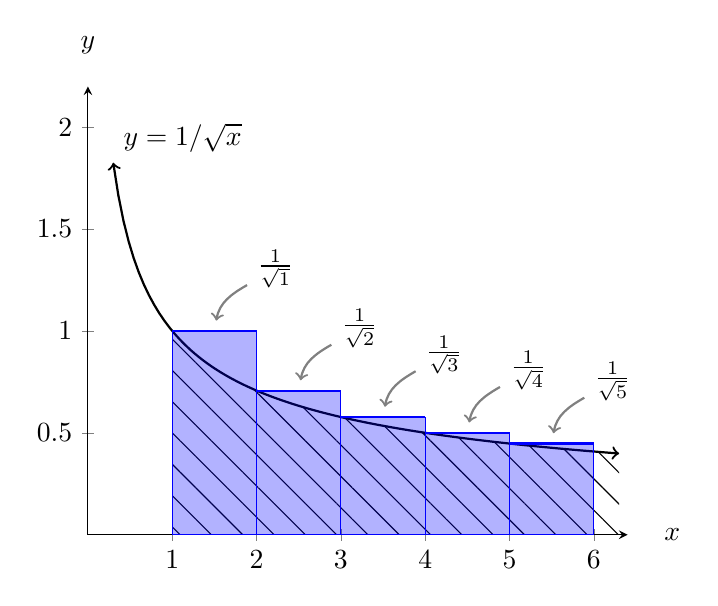
\begin{tikzpicture}
	\begin{axis}[
			twoDaxis,
			xmin = 0,
			xmax = 6.4,
			ymin = 0,
			ymax = 2.2,
			xtick = {1,2,3,4,5,6},
			% xticklabels = {$a$},
			% ytick=\empty,
			xlabel = {$x$},
			area plot/.style={
					fill opacity=0.3,
					draw=blue,
					% dashed,
					fill=blue,
					mark=none,
				} % sets up the orange slice fill in stuff
		]
		\addplot[black, <->, domain=0.3:6.3,name path = curve, thick] {1/x^0.5} node [pos=0,above right] {$y=1/\sqrt{x}$};
		\addplot[draw = none, domain = 1:6.3, name path = floor] {0};
		\tikzmath {
			% set the number of rectangles (it's off by 1 but I don't care)
			\N = 5;
		}
		%set up the loop
		\pgfplotsinvokeforeach{1,...,\N} {
			\tikzmath{
				% calculate the current x value for each iteration (otherwise it acts weird) (the 4 is hard coded the width of theinterval and "#1" is like "i" in a C loop, it is "this iteration number")
				\currentx{#1} = #1;
				% cacluctate the current y value for each iteration (we use it multiple times so only calculate it once here)
				\currenty{#1} = 1/\currentx{#1}^0.5;
			}
			% plot the slice for this iteration by plotting the 4 coordinates of the square's vertices and use closedcycle to connect them, using the area plot style we set up earlier to color them orange and all that
			\addplot[blue, domain=\currentx{#1}:{\currentx{#1}+1},name path = A, thick] {\currenty{#1}} node [midway, pin={[pin distance=0.4cm, pin edge={<-, thick, solid, out=80, in=210},black]above right:$\frac{1}{\sqrt{\currentx{#1}}}$}] {};
			\addplot[area plot] (\currentx{#1},\currenty{#1}) -- (\currentx{#1}+1,\currenty{#1}) -- (\currentx{#1}+1,0) -- (\currentx{#1},0) -- cycle;
		}
		\addplot[pattern = {Lines[angle=135,distance=8pt,line width=.4pt]}] fill between [of=curve and floor, soft clip={domain=1:6.3}];
	\end{axis}
\end{tikzpicture}
\end{document}